\documentclass[12pt, titlepage]{article}

\usepackage{fullpage}
\usepackage[round]{natbib}
\usepackage{multirow}
\usepackage{booktabs}
\usepackage{tabularx}
\usepackage{graphicx}
\usepackage{float}
\usepackage{hyperref}
\hypersetup{
    colorlinks,
    citecolor=blue,
    filecolor=black,
    linkcolor=red,
    urlcolor=blue
}

%% Comments

\usepackage{color}

\newif\ifcomments\commentstrue %displays comments
%\newif\ifcomments\commentsfalse %so that comments do not display

\ifcomments
\newcommand{\authornote}[3]{\textcolor{#1}{[#3 ---#2]}}
\newcommand{\todo}[1]{\textcolor{red}{[TODO: #1]}}
\else
\newcommand{\authornote}[3]{}
\newcommand{\todo}[1]{}
\fi

\newcommand{\wss}[1]{\authornote{blue}{SS}{#1}} 
\newcommand{\plt}[1]{\authornote{magenta}{TPLT}{#1}} %For explanation of the template
\newcommand{\an}[1]{\authornote{cyan}{Author}{#1}}

%% Common Parts

\newcommand{\progname}{ProgName} % PUT YOUR PROGRAM NAME HERE
\newcommand{\authname}{Team \#, Team Name
\\ Student 1 name
\\ Student 2 name
\\ Student 3 name
\\ Student 4 name} % AUTHOR NAMES                  

\usepackage{hyperref}
    \hypersetup{colorlinks=true, linkcolor=blue, citecolor=blue, filecolor=blue,
                urlcolor=blue, unicode=false}
    \urlstyle{same}
                                


\newcounter{acnum}
\newcommand{\actheacnum}{AC\theacnum}
\newcommand{\acref}[1]{AC\ref{#1}}

\newcounter{ucnum}
\newcommand{\uctheucnum}{UC\theucnum}
\newcommand{\uref}[1]{UC\ref{#1}}

\newcounter{mnum}
\newcommand{\mthemnum}{M\themnum}
\newcommand{\mref}[1]{M\ref{#1}}

\begin{document}

\title{Module Guide for \progname{}} 
\author{\authname}
\date{\today}

\maketitle

\pagenumbering{roman}

\section{Revision History}

\begin{tabularx}{\textwidth}{p{3cm}p{2cm}X}
\toprule {\bf Date} & {\bf Version} & {\bf Notes}\\
\midrule
01/16/2025 & 0.0 & Revision 0\\
\bottomrule
\end{tabularx}

\newpage

\section{Reference Material}

This section records information for easy reference.

\subsection{Abbreviations and Acronyms}

\renewcommand{\arraystretch}{1.2}
\begin{tabular}{l l} 
  \toprule		
  \textbf{symbol} & \textbf{description}\\
  \midrule 
  AC & Anticipated Change\\
  DAG & Directed Acyclic Graph \\
  DNN & Deep Neural Network \\
  M & Module \\
  MG & Module Guide \\
  OS & Operating System \\
  R & Requirement\\
  SC & Scientific Computing \\
  SRS & Software Requirements Specification\\
  TPG & Tangled Program Graphs\\
  UC & Unlikely Change \\
  % \wss{etc.} & \wss{...}\\
  \bottomrule
\end{tabular}\\

\newpage

\tableofcontents

\listoftables

\listoffigures

\newpage

\pagenumbering{arabic}

\section{Introduction}

Decomposing a system into modules is a commonly accepted approach to developing
software.  A module is a work assignment for a programmer or programming
team~\citep{ParnasEtAl1984}.  We advocate a decomposition
based on the principle of information hiding~\citep{Parnas1972a}.  This
principle supports design for change, because the ``secrets'' that each module
hides represent likely future changes.  Design for change is valuable in SC,
where modifications are frequent, especially during initial development as the
solution space is explored.  

Our design follows the rules layed out by \citet{ParnasEtAl1984}, as follows:
\begin{itemize}
\item System details that are likely to change independently should be the
  secrets of separate modules.
\item Each data structure is implemented in only one module.
\item Any other program that requires information stored in a module's data
  structures must obtain it by calling access programs belonging to that module.
\end{itemize}

After completing the first stage of the design, the Software Requirements
Specification (SRS), the Module Guide (MG) is developed~\citep{ParnasEtAl1984}. The MG
specifies the modular structure of the system and is intended to allow both
designers and maintainers to easily identify the parts of the software.  The
potential readers of this document are as follows:

\begin{itemize}
\item New project members: This document can be a guide for a new project member
  to easily understand the overall structure and quickly find the
  relevant modules they are searching for.
\item Maintainers: The hierarchical structure of the module guide improves the
  maintainers' understanding when they need to make changes to the system. It is
  important for a maintainer to update the relevant sections of the document
  after changes have been made.
\item Designers: Once the module guide has been written, it can be used to
  check for consistency, feasibility, and flexibility. Designers can verify the
  system in various ways, such as consistency among modules, feasibility of the
  decomposition, and flexibility of the design.
\end{itemize}

The rest of the document is organized as follows. Section
\ref{SecChange} lists the anticipated and unlikely changes of the software
requirements. Section \ref{SecMH} summarizes the module decomposition that
was constructed according to the likely changes. Section \ref{SecConnection}
specifies the connections between the software requirements and the
modules. Section \ref{SecMD} gives a detailed description of the
modules. Section \ref{SecTM} includes two traceability matrices. One checks
the completeness of the design against the requirements provided in the SRS. The
other shows the relation between anticipated changes and the modules. Section
\ref{SecUse} describes the use relation between modules.

\section{Anticipated and Unlikely Changes} \label{SecChange}

This section lists possible changes to the system. According to the likeliness
of the change, the possible changes are classified into two
categories. Anticipated changes are listed in Section \ref{SecAchange}, and
unlikely changes are listed in Section \ref{SecUchange}.

\subsection{Anticipated Changes} \label{SecAchange}

Anticipated changes are the source of the information that is to be hidden
inside the modules. Ideally, changing one of the anticipated changes will only
require changing the one module that hides the associated decision. The approach
adapted here is called design for
change.

\begin{description}
  \item[\refstepcounter{acnum} \actheacnum \label{acOutput1}:] Support for additional MuJoCo environments.
  \item[\refstepcounter{acnum} \actheacnum \label{acOutput2}:] Simulation support for all types of operating systems.
  \item[\refstepcounter{acnum} \actheacnum \label{acOutput3}:] Comprehensive logging across all of TPG's components.
  \item[\refstepcounter{acnum} \actheacnum \label{acVerif1}:] Extensive testing and checks for newly published code.
  \item[\refstepcounter{acnum} \actheacnum \label{acVerify2}:] Refactoring old and unstructured components.
  \item[\refstepcounter{acnum} \actheacnum \label{acInput}:] Format of inputting experimental parameters.
  \item[\refstepcounter{acnum} \actheacnum \label{acControl}:] Shift to a different dependency management tool such as CMake.
\end{description}

\subsection{Unlikely Changes} \label{SecUchange}

The module design should be as general as possible. However, a general system is
more complex. Sometimes this complexity is not necessary. Fixing some design
decisions at the system architecture stage can simplify the software design. If
these decision should later need to be changed, then many parts of the design
will potentially need to be modified. Hence, it is not intended that these
decisions will be changed.

\begin{description}
  \item[\refstepcounter{ucnum} \uctheucnum \label{ucControl1}:] Migration of TPG's implementation to a different language.
  \item[\refstepcounter{ucnum} \uctheucnum \label{ucControl2}:] Refactoring the flow of task initialization and generation.
  \item[\refstepcounter{ucnum} \uctheucnum \label{ucVerify1}:] Transitioning away from Github Actions to other CI/CD platforms.
  \item[\refstepcounter{ucnum} \uctheucnum \label{ucControl3}:] Replacement of MPI as the distributed computing framework.
  \item[\refstepcounter{ucnum} \uctheucnum \label{ucControl4}:] Changing of communication protocol between different components such as gRPC.
\end{description}

\section{Module Hierarchy} \label{SecMH}

This section provides an overview of the module design. Modules are summarized
in a hierarchy decomposed by secrets in Table \ref{TblMH}. The modules listed
below, which are leaves in the hierarchy tree, are the modules that will
actually be implemented.

\begin{description}
\item [\refstepcounter{mnum} \mthemnum \label{mHH}:] Hardware Hiding Module
\item [\refstepcounter{mnum} \mthemnum \label{mClassicControl}:] Classic Control Module
\item [\refstepcounter{mnum} \mthemnum \label{mMuJoCo}:] MuJoCo Module
\item [\refstepcounter{mnum} \mthemnum \label{mVisualization}:] Visualization Module
\item [\refstepcounter{mnum} \mthemnum \label{mLogging}:] Logging Module
\item [\refstepcounter{mnum} \mthemnum \label{mExperiment}:] TPG Experiment Module
\end{description}


\begin{table}[h!]
\centering
\begin{tabular}{p{0.3\textwidth} p{0.6\textwidth}}
\toprule
\textbf{Level 1} & \textbf{Level 2}\\
\midrule

{Hardware-Hiding Module} & N/A \\
\midrule

\multirow{4}{0.3\textwidth}{Behaviour-Hiding Module} & Classic Control Module \\
& MuJoCo Module\\
& Visualization Module\\
& Logging Module\\
\midrule

\multirow{2}{0.3\textwidth}{Software Decision Module} & {TPG Experiment Module}\\
& Framework Module\\
\bottomrule

\end{tabular}
\caption{Module Hierarchy}
\label{TblMH}
\end{table}

\section{Connection Between Requirements and Design} \label{SecConnection}

The design of the system is intended to satisfy the requirements developed in
the SRS. In this stage, the system is decomposed into modules. The connection
between requirements and modules is listed in Table~\ref{TblRT}.

\section{Module Decomposition} \label{SecMD}

Modules are decomposed according to the principle of ``information hiding''
proposed by \citet{ParnasEtAl1984}. The \emph{Secrets} field in a module
decomposition is a brief statement of the design decision hidden by the
module. The \emph{Services} field specifies \emph{what} the module will do
without documenting \emph{how} to do it. For each module, a suggestion for the
implementing software is given under the \emph{Implemented By} title. If the
entry is \emph{OS}, this means that the module is provided by the operating
system or by standard programming language libraries.  \emph{\progname{}} means the
module will be implemented by the \progname{} software.

Only the leaf modules in the hierarchy have to be implemented. If a dash
(\emph{--}) is shown, this means that the module is not a leaf and will not have
to be implemented.

\subsection{Hardware Hiding Modules (\mref{mHH})}

\begin{description}
\item[Secrets:]The data structure and algorithm used to implement the virtual
  hardware.
\item[Services:]Serves as a virtual hardware used by the rest of the
  system. This module provides the interface between the hardware and the
  software. So, the system can use it to display outputs or to accept inputs.
\item[Implemented By:] OS
\end{description}

\subsection{Behaviour-Hiding Module}

\begin{description}
\item[Secrets:]The contents of the required behaviours.
\item[Services:]Includes programs that provide externally visible behaviour of
  the system as specified in the software requirements specification (SRS)
  documents. This module serves as a communication layer between the
  hardware-hiding module and the software decision module. The programs in this
  module will need to change if there are changes in the SRS.
\item[Implemented By:] --
\end{description}

\subsubsection{Classic Control Module (\mref{mClassicControl})}

\begin{description}
\item[Secrets:]Classic Control's data structures (such as disReset, actionTrace, etc…).
\item[Services:]Provides an interface between TPG and established for the classic control environments to allow for simulation and comparisons.
\item[Implemented By:] Existing TPG framework
\item[Type of Module:] Abstract Object
\end{description}

\subsubsection{MuJoCo Module (\mref{mMuJoCo})}

\begin{description}
\item[Secrets:]MuJoCo's data structures (such as mjModel, mjData, etc…).
\item[Services:]Provides an interface between TPG and MuJoCo to allow for simulation within MuJoCo-based experiments.
\item[Implemented By:] \progname{}
\item[Type of Module:] Abstract Object
\end{description}

\subsubsection{Visualization Module (\mref{mVisualization})}

\begin{description}
\item[Secrets:]Output logs from tpg*.std files.
\item[Services:]Provides the visualization of the experiment being run. Extract metrics from logs, aggregate the metrics, plot, and combine them into a singular PDF.
\item[Implemented By:] \progname{}
\item[Type of Module:] Abstract Object
\end{description}


\subsubsection{Logging Module  (\mref{mLogging})}

\begin{description}
\item[Secrets:] Generate logs containing experiment execution data, performance metrics, and debug information.
\item[Services:] Provides comprehensive logging functionality across all TPG components to be utilized by the visualization module
\item[Implemented By:] \progname{}
\item[Type of Module:] Abstract Object
\end{description}

% \subsubsection{Etc.}


\subsection{Software Decision Module}

\begin{description}
\item[Secrets:] The design decision based on mathematical theorems, physical
  facts, or programming considerations. The secrets of this module are
  \emph{not} described in the SRS.
\item[Services:] Includes data structure and algorithms used in the system that
  do not provide direct interaction with the user. 
  % Changes in these modules are more likely to be motivated by a desire to
  % improve performance than by externally imposed changes.
\item[Implemented By:] --
\end{description}

\subsubsection{TPG Experiment Module (\mref{mExperiment})}
\begin{description}
  \item[Secrets:] Task parameters, team structures and decision making policies.
  \item[Services:] Provides functionality to manage and evolve policies, evaluation of different tasks, and track on-going experiments
  \item[Implemented By:] \progname{}
  \end{description}

\section{Traceability Matrix} \label{SecTM}

This section shows two traceability matrices: between the modules and the
requirements and between the modules and the anticipated changes.

% the table should use mref, the requirements should be named, use something
% like fref
\begin{table}[H]
\centering
\begin{tabular}{p{0.2\textwidth} p{0.6\textwidth}}
\toprule
\textbf{Req.} & \textbf{Modules}\\
\midrule
FR-1 & \mref{mMuJoCo}\\
FR-2 & \mref{mVisualization}\\
FR-3 & \mref{mLogging}\\
FR-4 & \mref{mHH}, \mref{mLogging}, \mref{mExperiment}\\
FR-5 & \mref{mClassicControl}, \mref{mMuJoCo}, \mref{mLogging}, \mref{mExperiment}\\
FR-6 & \mref{mClassicControl}, \mref{mMuJoCo}, \mref{mVisualization}, \mref{mLogging}, \mref{mExperiment}\\
FR-7 & \mref{mLogging}, \mref{mExperiment}\\
FR-8 & \mref{mClassicControl}, \mref{mMuJoCo}, \mref{mVisualization}\\
\bottomrule
\end{tabular}
\caption{Trace Between Requirements and Modules}
\label{TblRT}
\end{table}

\begin{table}[H]
  \centering
  \begin{tabular}{|c|c|c|} \hline 
  \toprule
  Anticipated Change
  & Modules & Module Numbers
  \\
  \midrule
  AC1
  & MuJoCo & \mref{mMuJoCo}
  \\
  AC2
  & Hardware, Visualization & \mref{mHH}, \mref{mVisualization}
  \\
  AC3
  & Hardware, Logging & \mref{mHH}, \mref{mLogging}
  \\
  AC4
  & Classic Control, MuJoCo, TPG Experiment  & \mref{mClassicControl}, \mref{mMuJoCo}, \mref{mExperiment}
  \\
  AC5
  & Classic Control, TPG Experiment  & \mref{mClassicControl}, \mref{mExperiment}
  \\
  AC6
  & Hardware, Classic Control, MuJoCo & \mref{mHH}, \mref{mClassicControl}, \mref{mMuJoCo}
  \\
  AC7
  & Visualization, Logging, TPG Experiment & \mref{mVisualization}, \mref{mLogging}, \mref{mExperiment}
  \\
  \bottomrule
  \end{tabular}
  \caption{Trace Between Anticipated Changes and Modules}
  \label{TblACT}
  \end{table}

\section{Use Hierarchy Between Modules} \label{SecUse}

In this section, the uses hierarchy between modules is
provided. \citet{Parnas1978} said of two programs A and B that A {\em uses} B if
correct execution of B may be necessary for A to complete the task described in
its specification. That is, A {\em uses} B if there exist situations in which
the correct functioning of A depends upon the availability of a correct
implementation of B.  Figure \ref{FigUH} illustrates the use relation between
the modules. It can be seen that the graph is a directed acyclic graph
(DAG). Each level of the hierarchy offers a testable and usable subset of the
system, and modules in the higher level of the hierarchy are essentially simpler
because they use modules from the lower levels.

% \wss{The uses relation is not a data flow diagram.  In the code there will often
% be an import statement in module A when it directly uses module B.  Module B
% provides the services that module A needs.  The code for module A needs to be
% able to see these services (hence the import statement).  Since the uses
% relation is transitive, there is a use relation without an import, but the
% arrows in the diagram typically correspond to the presence of import statement.}

% \wss{If module A uses module B, the arrow is directed from A to B.}

\begin{figure}[H]
\centering
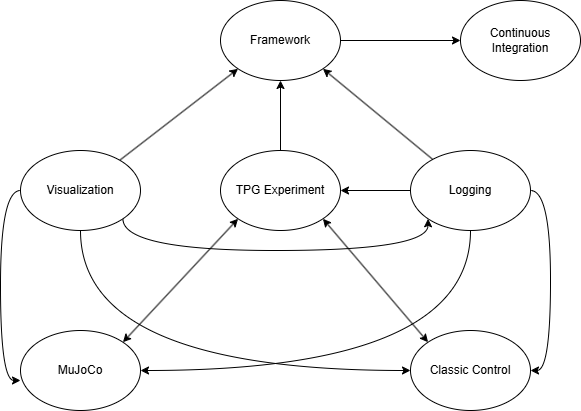
\includegraphics[width=0.7\textwidth]{use_hierarchy.png}
\caption{Use hierarchy among modules}
\label{FigUH}
\end{figure}

%\section*{References}

% \section{User Interfaces}

% \wss{Design of user interface for software and hardware.  Attach an appendix if
% needed. Drawings, Sketches, Figma}

% \section{Design of Communication Protocols}

% \wss{If appropriate}

\section{Timeline}

The capstone project's timeline will correspond to the main goals that have been outlined. The work has been split between the different modules with respective deadlines so that the team can work on separate modules concurrently. The deadlines have been set to help track progress and establish expectations. 

\begin{center}
    \begin{table}
    \centering
    \begin{tabular}{p{0.6\textwidth} p{0.2\textwidth} p{0.2\textwidth}}


         \textbf{Module}&  \textbf{Related members}& \textbf{Deadline}\\ \hline 
         Classic Control (7.2.1) - Develop the core control functionalities&  Whole Team & Jan 15, 2024\\ \hline 
         MuJoCo (7.2.2) - Integrate the TPG framework with MuJoCo environments, ensuring compatibility and validation.&  Whole Team & Jan 31, 2024\\ \hline 
         Visualization (7.2.3) - Implement visualization functionality with tangible data such as 
        graphs, charts, video playback,realtime simulation to view results.
         &  Edward & Jan 25, 2024\\ \hline 
         Logging (7.2.4) - Implement functionality to capture key info and debug information throughout framework &   Whole Team & Jan 31, 2024\\ \hline 
         TPG Experiment (7.2.5) - Design and execute experiments to test the TPG framework performance across various scenarios& Edward, Cyruss & Jan 20, 2024\\ \hline 
         Framework (7.2.6) - should create functionality to authenticate a user using auth0&  Cyruss, Mark & Jan 25, 2024\\ \hline 
         Continuous Integration  (7.2.7) - Establish a CI pipeline for automatic linting, project building, and unit testing to ensure code quality and integration stability &  Calvyn, Richard& Jan 31, 2024\\ \hline 
    \end{tabular}
    \caption{Timeline for each module}
    \label{tab:my_label}
\end{table}
\end{center}

\bibliographystyle {plainnat}
\bibliography{../../../refs/References}

\newpage{}

\end{document}